% LTeX: language=es
\documentclass[a4paper, 11pt]{article}
\usepackage{comment} 
\usepackage{fullpage} 
\usepackage{graphicx}
\usepackage[spanish]{babel}
\usepackage[utf8]{inputenc}
\usepackage{float}
\usepackage{MnSymbol,wasysym}
\usepackage{tikz}
\usetikzlibrary{positioning, arrows.meta, fit, backgrounds, shapes.geometric}
\pgfdeclarelayer{background}
\pgfsetlayers{ background, main }
\usepackage{xcolor}
\usepackage{parskip}
\usepackage{microtype}
\setlength{\emergencystretch}{3em}
\usepackage{listings}
\usepackage{dirtree}

% ─── Listings colors ─────────────────────────────────────────────────────────
\definecolor{bashbg}{HTML}{1E1E2E}
\definecolor{bashfg}{HTML}{CDD6F4}
\definecolor{bashgreen}{HTML}{A6E3A1}
\definecolor{clkw}{HTML}{0550AE}
\definecolor{clstr}{HTML}{116329}
\definecolor{clcmt}{HTML}{6E7781}
\definecolor{clbuiltin}{HTML}{8250DF}
\definecolor{clframe}{HTML}{CCCCCC}

% ─── Listings base (frame + spacing) ──────────────────────────────────────────
\lstset{
  frame=single,
  framerule=0.4pt,
  rulecolor=\color{clframe},
  aboveskip=1em,
  belowskip=1em,
  breaklines=true,
  breakatwhitespace=true,
  columns=flexible,
}

% ─── Bash style ───────────────────────────────────────────────────────────────
\lstdefinestyle{bash}{
  language=bash,
  basicstyle=\ttfamily\small,
  keywordstyle=\color{clkw}\bfseries,
  stringstyle=\color{clstr},
  commentstyle=\color{clcmt}\itshape,
  showstringspaces=false,
  breaklines=true,
  breakatwhitespace=true,
}

% ─── Nix language + style ─────────────────────────────────────────────────────
\lstdefinelanguage{nix}{
  keywords={let, in, rec, with, inherit, if, then, else, assert, import,
            null, true, false},
  morekeywords=[2]{builtins, pkgs, lib, config, options},
  sensitive=true,
  comment=[l]{\#},
  morecomment=[s]{/*}{*/},
  morestring=[b]",
  morestring=[b]'',
}

\lstdefinestyle{nix}{
  language=nix,
  basicstyle=\ttfamily\small,
  keywordstyle=\color{clkw}\bfseries,
  keywordstyle=[2]\color{clbuiltin},
  stringstyle=\color{clstr},
  commentstyle=\color{clcmt}\itshape,
  showstringspaces=false,
  breaklines=true,
  breakatwhitespace=true,
}

% ─── Terraform/HCL language + style ──────────────────────────────────────────
\lstdefinelanguage{terraform}{
  keywords={resource, variable, output, module, provider, data, locals,
            terraform, required_providers, backend, for_each, count,
            dynamic, content, lifecycle, depends_on},
  morekeywords=[2]{true, false, null, var, local, module, each, self, path},
  sensitive=true,
  comment=[l]{\#},
  morecomment=[s]{/*}{*/},
  morestring=[b]",
}

\lstdefinestyle{terraform}{
  language=terraform,
  basicstyle=\ttfamily\small,
  keywordstyle=\color{clkw}\bfseries,
  keywordstyle=[2]\color{clbuiltin},
  stringstyle=\color{clstr},
  commentstyle=\color{clcmt}\itshape,
  showstringspaces=false,
  breaklines=true,
  breakatwhitespace=true,
}

\definecolor{linkblue}{HTML}{1a0dab}
\usepackage[
    colorlinks=true,
    linkcolor=linkblue,
    filecolor=linkblue,
    urlcolor=linkblue,
    citecolor=linkblue,
    pdfdisplaydoctitle=true,
]{hyperref}
\usepackage{csquotes}
\usepackage[backend=bibtex, style=numeric, sorting=none]{biblatex}
\addbibresource{refs.bib}

\begin{document}

\begin{titlepage}
    \vspace*{\fill}

    \begin{center}
        {\huge \textbf{Trabajo Tutelado AII: \\ [0.5cm] Infraestructura declarativa reproducible usando OpenTofu y NixOS}}
    \end{center}

    \vspace*{\fill}

    \begin{flushright}
        \textit{Autores:} \\
        Mario Lamas Angeriz (\href{mailto:m.lamasa@udc.es}{m.lamasa@udc.es}) \\
        Alexandre Borrazás Mancebo (\href{mailto:alexandre.bmancebo@udc.es}{alexandre.bmancebo@udc.es}) \\[0.5em]
        \href{https://github.com/alexborrazasm/terraform-proxmox-nixos-infra}{Repositorio en GitHub} \\
    \end{flushright}
\end{titlepage}

\newpage
\tableofcontents
\newpage

\section{Propuesta}

Aprender más sobre \textbf{Infrastructure as Code} (\textbf{IaC}) usando herramientas
como \textbf{Terraform}~\cite{terraform} o \textbf{OpenTofu}~\cite{opentofu} que permiten describir y desplegar
infraestructura de forma declarativa, mientras que \textbf{NixOS}~\cite{nixos} proporciona un
sistema operativo completamente reproducible cuya configuración también se define
mediante código.

Este trabajo propone explorar la integración de ambas tecnologías para crear una 
infraestructura completamente declarativa, donde tanto la creación de recursos 
como la configuración del sistema operativo estén definidas en repositorios 
versionados (\href{https://github.com/alexborrazasm/terraform-proxmox-nixos-infra}{\texttt{GitHub}}).

\section{Objetivos}

El objetivo principal del trabajo es diseñar e implementar una plataforma de 
infraestructura reproducible basada en principios de \textbf{Infrastructure as Code}.

\begin{itemize} 
  \item Estudiar el paradigma de infraestructura declarativa.
  \item Analizar el funcionamiento de \textbf{Terraform}~\cite{terraform} y \textbf{OpenTofu}~\cite{opentofu} para la provisión de recursos.
  \item Analizar el modelo de configuración declarativa de \textbf{NixOS}~\cite{nixos}.
  \item Diseñar una arquitectura donde \textbf{Terraform}~\cite{terraform} o \textbf{OpenTofu}~\cite{opentofu} gestione
    la infraestructura y \textbf{NixOS}~\cite{nixos} configure los sistemas.
  \item Implementar un entorno reproducible donde la infraestructura pueda desplegarse 
    automáticamente a partir del código.
  \item Evaluar las ventajas y limitaciones del enfoque propuesto.
\end{itemize} 

\section{Hardware empleado}

Para la realización del proyecto contamos con un servidor rack \textbf{Dell} cedido 
por un amigo, cuyas especificaciones técnicas relevantes para el proyecto son las siguientes:

\begin{itemize}
    \item \textbf{CPU}: Intel\textsuperscript{\textregistered} Xeon\textsuperscript{\textregistered} E5-2420 v2 @ 2.20GHz --- 12 cores (1 socket)
    \item \textbf{RAM}: 32 GiB
    \item \textbf{Almacenamiento}: 6 discos duros extraíbles \textit{hot-swappable} de 136 GB cada uno, configurados en \textbf{RAID 1+0}.
\end{itemize}

\section{Tecnologías usadas}

Para la realización del proyecto decidimos emplear las siguientes tecnologías:

\begin{itemize}
  \item \textbf{Proxmox VE}~\cite{proxmox}: plataforma de virtualización open-source que utilizamos como
    hipervisor para la gestión de nuestras máquinas virtuales.
  \item \textbf{pfSense}~\cite{pfsense}: firewall y router virtualizado que empleamos para la gestión de las redes del proyecto.
  \item \textbf{Tailscale}~\cite{tailscale}: VPN de configuración cero utilizada como acceso remoto de respaldo.
  \item \textbf{OpenTofu}~\cite{opentofu}: fork de Terraform open-source (sus ficheros de configuración son compatibles),
    herramienta de IaC que empleamos para la declaración y asignación de recursos de nuestras máquinas virtuales.
  \item \textbf{NixOS}~\cite{nixos}: distribución de Linux que emplea el gestor de paquetes Nix, gracias a su configuración
    declarativa nos permite desplegar en las máquinas virtuales todo tipo de servicios de forma sencilla y automatizada.
  \item \textbf{nixos-anywhere}~\cite{nixos-anywhere}: herramienta de instalación de NixOS, nos permite realizar la instalación del SO
    de forma remota mediante \texttt{ssh} y de forma completamente automatizada.
  \item \textbf{Colmena}~\cite{colmena}: tras la primera build de los sistemas de NixOS, Colmena nos permite realizar cambios sobre
    el SO (mientras este se ejecuta) de forma remota y sencilla sin necesidad de reinstalar.
  \item \textbf{agenix}~\cite{agenix}: paquete que permite la gestión de secretos mediante cifrado
    \texttt{age}~\cite{age}, nos permite crear secretos y subirlos a un repositorio sin miedo a exponer información sensible.
  \item \textbf{Docker}~\cite{docker}: mediante la configuración en NixOS, podemos desplegar servicios
    sobre Docker en boot lanzándolos de forma automatizada.
  \item \textbf{Caddy}~\cite{caddy}: servidor web y proxy inverso con gestión automática de certificados TLS.
  \item \textbf{Nginx}~\cite{nginx}: servidor HTTP utilizado en los workers para servir páginas de índice.
  \item \textbf{Prometheus}~\cite{prometheus}: sistema de monitorización y base de datos de series temporales.
  \item \textbf{Grafana}~\cite{grafana}: plataforma de observabilidad para visualización de métricas.
  \item \textbf{WireGuard}~\cite{wireguard}: protocolo VPN moderno y seguro para el acceso remoto a la red.
  \item \textbf{Disko}~\cite{disko}: herramienta de particionado declarativo de discos para NixOS.
  \item \textbf{fail2ban}~\cite{fail2ban}: software de prevención de intrusiones que protege los servicios SSH.
\end{itemize}

\section{Diagrama de red y estructura base}

En primer lugar, instalamos Proxmox VE~\cite{proxmox} como hipervisor en el 
servidor para poder virtualizar las máquinas necesarias para el proyecto.

A continuación, decidimos definir la estructura de red, y equipos/contenedores 
a crear.

Antes de empezar a desarrollar el código de IaC, era necesario tener una red 
funcional que nos permitiese trabajar con las máquinas virtuales de forma cómoda 
y segura.

Para ello reemplazamos el router de nuestro piso por un router virtualizado con 
\textbf{pfSense}~\cite{pfsense} y creamos 2 contenedores LXC~\cite{proxmox-lxc} 
Debian para las VPN, uno con \textbf{Tailscale}~\cite{tailscale} y otro con
\textbf{WireGuard}~\cite{wireguard}. El \textbf{Tailscale} está de \textit{fallback}, es
decir, por si el WireGuard falla, siempre tenemos una forma de acceder a la red 
de forma remota.

Ahora en cuanto a la red, decidimos crear 3 redes, como se puede ver en la 
\autoref{fig:red}, se creó una red \textbf{DMZ} para poder aislar las máquinas y 
reproducir de forma más fiable una red empresarial de producción. La red \textbf{LAN} 
es la red habitual que todos tenemos en casa, aquí simulamos la intranet de una 
organización y la \textbf{WAN} representa internet. 

Como solo disponemos de 1 dirección IP en el router hemos redirigido el 
puerto \texttt{3478/udp} hacia nuestro WireGuard y además los puertos 
\texttt{80/tcp}/\texttt{443/tcp}/\texttt{443/udp} hacia nuestro \textit{reverse 
proxy}, en este caso \textbf{Caddy}, que permite el acceso externo a las webs.

El resto de las máquinas de la red están aisladas frente accesos no permitidos, 
solo se puede acceder a ellas desde la red LAN o la VPN, y además solo aceptan 
conexiones \texttt{ssh} con autenticación por clave pública.

Una vez con esto establecido podíamos centrarnos en el desarrollo del proyecto 
con los principios de IaC.

\begin{figure}[H]
  \centering
  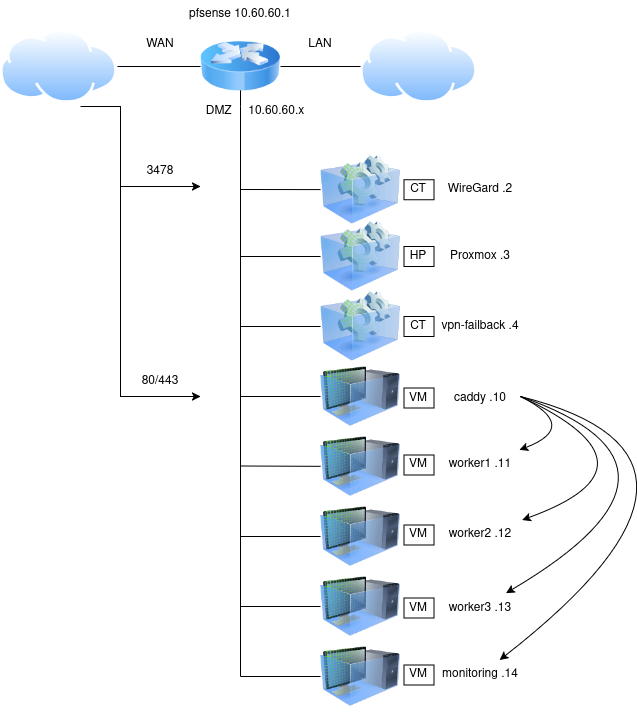
\includegraphics[width=0.7\textwidth]{./figures/networking.png}
  \caption{Esquema de red}\label{fig:red}
\end{figure}

\section{Estructura del proyecto}

Organizamos el proyecto en 3 carpetas:

\dirtree{%
.1 ..
.2 grafana.
.3 dashboard.json.
.3 load-dashboard.sh.
.2 nixos.
.3 deploy-new-host.sh.
.3 first-deploy.sh.
.3 flake.lock.
.3 flake.nix.
.3 hosts.
.4 caddy.
.5 default.nix.
.5 disk-config.nix.
.5 hardware-configuration.nix.
.4 monitoring.
.5 \ldots.
.4 worker1.
.5 \ldots.
.4 worker2.
.5 \ldots.
.4 worker3.
.5 \ldots.
.3 modules.
.4 caddy-config.
.5 Caddyfile.
.4 caddy.nix.
.4 common.nix.
.4 ddns.nix.
.4 docker.nix.
.4 fail2ban.nix.
.4 grafana.nix.
.4 neovim.nix.
.4 nginx-indexes.
.5 \ldots.
.4 nginx\_worker.nix.
.4 node\_exporter.nix.
.4 prometheus.nix.
.4 ssh.nix.
.4 users.nix.
.4 utils.nix.
.3 secrets.
.4 cf-token.age.
.4 grafana-admin-password.age.
.4 grafana-secret-key.age.
.4 secrets.nix.
.2 terraform.
.3 main.tf.
.3 tofu.sh.
.3 variables.tf.
}

\begin{itemize}
  \item \texttt{nixos}: dentro de esta carpeta se guardan todos los archivos de 
    configuración relacionados con el sistema operativo de los equipos.
  \item \texttt{terraform}: aquí mantenemos la declaración de asignación de 
    recursos a cada máquina (número CPU, memoria RAM, disco, red, etc.).
  \item \texttt{grafana}: guardamos un script y el dashboard para cargarlo en la 
    máquina correspondiente. 
\end{itemize}

\section{Desarrollo del proyecto}

\subsection{Configuraciones iniciales}

En primer lugar, se llevó a cabo la configuración de un router \textbf{pfSense}~\cite{pfsense} 
virtualizado, lo que nos permitió una gestión eficiente de las redes y su monitorización.

A continuación, se configuró un acceso remoto mediante \textbf{Tailscale}~\cite{tailscale}; 
sin embargo, esta solución únicamente permite el acceso de uno de los integrantes del equipo 
a la red. Por ello, se desplegó una segunda VPN basada en \textbf{WireGuard}~\cite{wireguard}, 
que posibilita el acceso remoto a ambos miembros del equipo de forma simultánea.

Cabe destacar que Tailscale se instaló como solución provisional para disponer de acceso 
inmediato mientras se investigaba y configuraba correctamente WireGuard, permaneciendo 
operativo una vez finalizado dicho proceso como backup. 

\subsection{Declaración de los recursos}

Inicialmente, se optó por utilizar \textbf{Terraform}~\cite{terraform} para la declaración 
de recursos; sin embargo, tras investigar y comparar con \textbf{OpenTofu}~\cite{opentofu}, 
se decidió migrar a esta última debido a su naturaleza completamente open-source, su comunidad 
activa y su desarrollo continuo. Cabe destacar que ambas herramientas son totalmente compatibles 
entre sí, ya que OpenTofu es un \textit{fork} directo de Terraform, por lo que comparten la 
misma sintaxis y ecosistema de proveedores. Esto garantiza además una mejor integración con 
otras herramientas de código abierto como \textbf{NixOS}~\cite{nixos}.

Para que OpenTofu pueda interactuar con el hipervisor, es necesario configurar el proveedor 
de Proxmox en el archivo \texttt{main.tf}. En concreto, se utiliza el proveedor 
\textbf{telmate/proxmox}~\cite{telmate}, que ofrece soporte para la API de Proxmox y permite 
gestionar recursos como máquinas virtuales y contenedores LXC de forma declarativa. 
La autenticación se realiza mediante un \textbf{API Token}, evitando así el uso de 
credenciales de superusuario (\texttt{root}).

\begin{lstlisting}[style=terraform]
provider "proxmox" {
  pm_api_url          = var.pm_api_url
  pm_api_token_id     = var.pm_api_token_id
  pm_api_token_secret = var.pm_api_token_secret
  pm_tls_insecure     = var.pm_tls_insecure
}

locals {
  vms = {
    caddy      = { vmid = 110, ip = "10.60.60.10", cores = 6, memory = 2048 }
    worker1    = { vmid = 111, ip = "10.60.60.11", cores = 1, memory = 2048 }
    worker2    = { vmid = 112, ip = "10.60.60.12", cores = 1, memory = 2048 }
    worker3    = { vmid = 113, ip = "10.60.60.13", cores = 1, memory = 2048 }
    monitoring = { vmid = 114, ip = "10.60.60.14", cores = 2, memory = 4096 }
  }
}

resource "proxmox_vm_qemu" "vms" {
  for_each = local.vms

  vmid        = each.value.vmid
  name        = "nixos-${each.key}"
  target_node = "pve"
  clone       = "debian-12-template"
  full_clone  = true
  scsihw      = "virtio-scsi-single"
  vm_state    = var.vm_state

  cpu {
    cores   = each.value.cores
    sockets = 1
    type    = "host"
  }

  memory = each.value.memory

  disks {
    scsi {
      scsi0 { disk    { storage = "local-lvm", size = "20G", iothread = true } }
      scsi1 { cloudinit { storage = "local-lvm" } }
    }
  }

  network {
    id     = 0
    model  = "virtio"
    bridge = "vmbr2" # DMZ
  }

  ipconfig0  = "ip=${each.value.ip}/24,gw=10.60.60.1"
  sshkeys    = var.sshkeys
  cipassword = var.cipassword
}
\end{lstlisting}

Para simplificar el uso de secretos, utilizamos un script \texttt{tofu.sh}, que es un
simple wrapper que carga las variables de entorno desde un archivo \texttt{.env},
y a continuación ejecuta el binario de OpenTofu con los parámetros necesarios 
pasados al script. De esta forma, no exponemos las credenciales de la API de
Proxmox en el código fuente. 

\subsection{Creación de la plantilla base}

Para la plantilla base se optó por una imagen \textbf{Debian 12} con soporte para 
\textbf{Cloud-init}~\cite{cloudinit}. Inicialmente se intentó utilizar una imagen 
de \textbf{Debian 13} instalada manualmente; sin embargo, se encontraron problemas de 
compatibilidad con Cloud-init relacionados con cambios en la configuración DNS introducidos 
en esta versión, lo que impedía el correcto aprovisionamiento de las máquinas virtuales. 
Tras investigar alternativas, se encontró la imagen oficial Cloud-init de Debian 12, 
que resultó plenamente funcional, por lo que se optó por ella en lugar de continuar 
con la instalación manual.

La configuración de \textbf{Cloud-init}, declarada desde OpenTofu, se encarga de establecer 
la red, el usuario y las claves SSH en cada máquina virtual durante el primer arranque. 
Además, se instala el gestor de paquetes \textbf{Nix}~\cite{nix}, necesario para el 
despliegue posterior de NixOS. De este modo, la plantilla queda lista para 
\textit{nixificarla}: con las claves SSH inyectadas automáticamente y Nix disponible, 
NixOS puede tomar el control del sistema sin intervención manual.

\subsection{Instalación de NixOS con nixos-anywhere}

Una vez que OpenTofu ha levantado las máquinas virtuales con Debian, utilizamos 
\textbf{nixos-anywhere}~\cite{nixos-anywhere} para realizar la transición a NixOS. 

A la primera máquina nos tenemos que conectar por SSH y sacar información del 
hardware para generar el archivo \texttt{hardware-configuration.nix} necesario 
para la instalación de NixOS.

De la siguiente forma:

\begin{lstlisting}[style=bash]
debian@template:~$ sudo $(which nix-shell) -p nixos-install-tools \
 --run "nixos-generate-config --no-filesystems --root /mnt"
debian@template:~$ cat /mnt/etc/nixos/hardware-configuration.nix
# Do not modify this file!  It was generated by 'nixos-generate-config'
# and may be overwritten by future invocations.  Please make changes
# to /etc/nixos/configuration.nix instead.
{ config, lib, pkgs, modulesPath, ... }:

{
  imports =
    [ (modulesPath + "/profiles/qemu-guest.nix")
    ];

  boot.initrd.availableKernelModules = [ "ata_piix" "uhci_hcd" "virtio_pci" "virtio_scsi" "sd_mod" "sr_mod" ];
  boot.initrd.kernelModules = [ ];
  boot.kernelModules = [ "kvm-intel" ];
  boot.extraModulePackages = [ ];

  nixpkgs.hostPlatform = lib.mkDefault "x86_64-linux";
}
\end{lstlisting}

Esta configuración nos sirve para definir el hardware de todas las máquinas virtuales 
NixOS, dado que todas ellas comparten el mismo hardware virtualizado.

Con el hardware definido, cada máquina se declara mediante \textbf{Nix}~\cite{nix} y se 
despliega utilizando \textbf{nixos-anywhere}~\cite{nixos-anywhere}, que carga una imagen 
mínima de NixOS en la RAM de la plantilla Debian, mediante SSH, y procede a instalar 
NixOS en el disco de cada máquina virtual, copiando la configuración declarada.

En este proceso se utiliza \textbf{disko}~\cite{disko} para el particionado declarativo 
de los discos, lo que nos permite definir la estructura de almacenamiento de 
forma sencilla y reproducible.

Las claves SSH de los hosts se generan localmente y se envían a cada máquina 
durante la instalación, garantizando que cada vez que se crean las máquinas
tengan siempre las claves SSH de host esperadas, garantizando así la idempotencia
y reproducibilidad de la infraestructura desde el primer despliegue. Además,
\textbf{agenix}~\cite{agenix} utiliza estas claves para descifrar los secretos necesarios 
para cada host. Si no se generan las claves de host de forma determinista, cada 
despliegue crearía nuevas claves, lo que invalidaría los secretos cifrados con 
las claves anteriores y rompería la reproducibilidad.

Posteriormente, cualquier cambio en la configuración de servicios, usuarios y
contenedores Docker se gestiona con \textbf{Colmena}~\cite{colmena}, lo que permite 
aplicar modificaciones en segundos sin necesidad de reiniciar la máquina ni reinstalar 
el sistema operativo.

\subsection{Gestión de cambios con Colmena}

Una vez realizado el despliegue inicial con \textbf{nixos-anywhere}, la 
herramienta encargada de gestionar el ciclo de vida de la configuración es 
\textbf{Colmena}~\cite{colmena}. 

A diferencia de \textbf{nixos-anywhere}, que instala el sistema desde cero, 
Colmena aplica cambios incrementales sobre máquinas ya en ejecución mediante SSH, 
sin necesidad de reiniciar ni reinstalar.

\subsubsection{Integración con el flake}

Colmena lee su configuración directamente del output \texttt{colmena} del \texttt{flake.nix}. 
Cada host se define con su dirección IP (\texttt{targetHost}), usuario de despliegue 
(\texttt{targetUser}) y su configuración NixOS, que es exactamente la misma que 
se usa en \texttt{nixosConfigurations}. 

En el archivo \texttt{flake.nix} la sección de Colmena tiene la siguiente forma:

\begin{lstlisting}[style=nix]
colmenaHive = colmena.lib.makeHive self.outputs.colmena;
    colmena = {
      meta = {
        nixpkgs = import nixpkgs { inherit system; };
        specialArgs = { inherit disko inputs; };
      };

      caddy = { name, nodes, pkgs, ... }: {
        deployment = {
          targetHost = "10.60.60.10";
          targetUser = builtins.getEnv "USER";

          # You can build on the target machine
          # buildOnTarget = true;
        };
        imports = caddyModules;
      };

      worker1 = { name, nodes, pkgs, ...}: {
        deployment = {
          targetHost = "10.60.60.11";
          targetUser = builtins.getEnv "USER";
        };
        imports = worker1Modules;
      };

      # worker2, worker3 ...

      monitoring = { name, nodes, pkgs, ...}: {
          deployment = {
              targetHost = "10.60.60.14";
              targetUser = builtins.getEnv "USER";
          };
          imports = monitoringModules;
      };

    };
\end{lstlisting}

\subsubsection{Flujo de trabajo habitual}

El flujo típico al modificar la configuración de uno o varios hosts es el siguiente:

\begin{enumerate}
  \item Se edita el módulo o archivo de host correspondiente en el repositorio.
  \item Se verifica que la configuración compila correctamente sin desplegar:
\begin{verbatim}
nix run github:zhaofengli/colmena -- build
\end{verbatim}
  \item Si la build es exitosa, se despliega el cambio. Para aplicarlo a un único host:
\begin{verbatim}
nix run github:zhaofengli/colmena -- apply --on <host> --impure
\end{verbatim}
  Para aplicarlo a toda la infraestructura de forma simultánea:
\begin{verbatim}
nix run github:zhaofengli/colmena -- apply --impure
\end{verbatim}
  \item Colmena construye la nueva generación del sistema en la máquina local (o 
    en el propio host si se configura despliegue remoto), 
    la transfiere por SSH y ejecuta \texttt{nixos-rebuild switch}, activando los 
    cambios en caliente.
\end{enumerate}

\subsubsection{Ventajas operativas}

El uso de Colmena frente a otros enfoques de despliegue aporta varias ventajas 
prácticas en nuestro contexto:

\begin{itemize}
  \item \textbf{Despliegue paralelo}: Colmena puede aplicar cambios a múltiples 
    hosts en paralelo, reduciendo el tiempo total de actualización de la 
    infraestructura completa.
  \item \textbf{Setup sencillo}: no requiere instalar ningún agente en los hosts 
    destino; únicamente necesita acceso SSH con el usuario y clave configurados 
    en \texttt{deployment}.
  \item \textbf{Consistencia}: aplicar la misma configuración varias veces 
    produce siempre el mismo resultado, sin efectos secundarios acumulativos.
\end{itemize}

\subsubsection{Configuración SSH para Colmena}

Para que Colmena pueda conectarse a cada host por SSH es necesario añadir 
una entrada en \texttt{\textasciitilde/.ssh/config} por cada máquina gestionada:

\begin{lstlisting}[style=bash]
Host 10.60.60.10
  IdentityFile ~/.ssh/<clave_ssh_ed25519>
Host 10.60.60.11
  IdentityFile ~/.ssh/<clave_ssh_ed25519>
Host 10.60.60.12
  IdentityFile ~/.ssh/<clave_ssh_ed25519>
Host 10.60.60.13
  IdentityFile ~/.ssh/<clave_ssh_ed25519>
Host 10.60.60.14
  IdentityFile ~/.ssh/<clave_ssh_ed25519>
\end{lstlisting}

De este modo Colmena selecciona automáticamente la clave correcta sin 
intervención manual durante el despliegue.

\subsection{Configuración de NixOS}

\subsubsection{Estructura del flake}

El punto de entrada de toda la configuración NixOS es el archivo \texttt{flake.nix}, que 
actúa como manifiesto del proyecto: declara las dependencias externas (inputs) y 
expone las configuraciones de cada host (outputs). Entre los inputs más relevantes 
se encuentran \texttt{nixpkgs} (el repositorio de paquetes de NixOS), \texttt{agenix}~\cite{agenix} 
(gestión de secretos), \texttt{disko}~\cite{disko} (particionado declarativo) y 
\texttt{colmena}~\cite{colmena} (despliegue remoto).

Cada host queda registrado dos veces: en el output de \texttt{nixosConfigurations} 
(usado por \textbf{nixos-anywhere} en el primer despliegue) y en el output de
\texttt{colmena} (usado para actualizaciones posteriores). Esto garantiza que la 
misma definición de sistema se emplee independientemente del mecanismo de despliegue.

\subsubsection{Módulos compartidos}

Para evitar la duplicación de configuración entre hosts, extraemos toda la 
lógica reutilizable en módulos bajo \texttt{nixos/modules/}. 

Cada host importa el subconjunto de módulos que necesita desde su \texttt{default.nix}.

\begin{itemize}
  \item common.nix
    
    Define la base común a todas las máquinas: zona horaria, locale, bootloader (\textbf{GRUB} en modo BIOS para compatibilidad con Proxmox), 
    y el conjunto mínimo de paquetes del sistema (\texttt{git}, \texttt{htop}, \texttt{curl}, etc.). También habilita \texttt{nix.settings.experimental-features} para soportar flakes.

  \item users.nix

    Declara los usuarios del sistema de forma centralizada. 
    Las claves SSH públicas de los administradores se incluyen directamente en la configuración, 
    de modo que cualquier máquina que importe este módulo acepta las mismas identidades desde el primer arranque. 
    Las contraseñas se deshabilitan forzando el acceso exclusivamente por certificado.

  \item ssh.nix

    Declara el tipo de las claves SSH y además endurece la configuración del demonio SSH: deshabilita el login con contraseña (\texttt{PasswordAuthentication = false}). 
    Combinado con \texttt{fail2ban}~\cite{fail2ban}, forman una firme defensa frente a accesos remotos no autorizados en cada máquina.

  \item fail2ban.nix

    Habilita el servicio \texttt{fail2ban}~\cite{fail2ban} con una jail para SSH que bloquea automáticamente direcciones IP tras varios intentos de autenticación fallidos. 
    La configuración de este módulo es común a todos los hosts.

  \item utils.nix y neovim.nix

    Agrupan herramientas de administración del sistema (\texttt{tmux}, \texttt{ripgrep}, \texttt{jq}, \texttt{wget}, etc.) 
    y la configuración personalizada de \textbf{Neovim} respectivamente, 
    disponibles en todas las máquinas para facilitar el trabajo de los administradores.

\end{itemize}

\subsubsection{Configuración de hosts}

Cada directorio bajo \texttt{nixos/hosts/<hostname>/} contiene tres archivos:

\begin{itemize}
  \item \texttt{hardware-configuration.nix}: generado a partir de la plantilla Debian; 
    captura los módulos del kernel necesarios para el hardware virtualizado de Proxmox (\texttt{virtio\_pci}, \texttt{virtio\_scsi}, etc.).
  \item \texttt{disk-config.nix}: define el esquema de particiones mediante \textbf{disko}~\cite{disko}. Usamos una tabla \textbf{GPT} con una partición de arranque BIOS y una partición raíz \texttt{ext4}.
  \item \texttt{default.nix}: configuración específica del host; importa los módulos necesarios, asigna el hostname y declara los servicios particulares de esa máquina.
\end{itemize}

\section{Servicios desplegados}

\subsection{Caddy (proxy inverso)}

La máquina \texttt{caddy} actúa como punto de entrada a toda la infraestructura. 
El módulo \texttt{caddy.nix} habilita el servicio \texttt{services.caddy} de NixOS apuntando a un \texttt{Caddyfile} 
personalizado ubicado en \texttt{modules/caddy-config/Caddyfile}. \textbf{Caddy}~\cite{caddy} gestiona automáticamente
los certificados TLS mediante \textbf{ACME}/\textbf{Let's Encrypt}~\cite{letsencrypt}, usando el token de \textbf{Cloudflare}~\cite{cloudflare}
(almacenado como secreto \texttt{age}~\cite{age}) para el challenge \textbf{DNS-01}, 
lo que permite obtener certificados incluso sin exponer el puerto \texttt{80} directamente.

El \texttt{Caddyfile} define los virtual hosts necesarios para enrutar el tráfico entrante hacia
los servicios internos de la red DMZ mediante proxy inverso, añadiendo cabeceras de seguridad y terminación TLS en este punto.

Además, hace de balanceador de carga entre los 3 workers, distribuyendo las peticiones entrantes de forma round-robin y permitiendo 
escalar horizontalmente los servicios desplegados en los workers.

\subsection{DDNS (ddns.nix)}

Dado que la IP pública del router puede cambiar, el módulo \texttt{ddns.nix} configura un servicio de \textbf{DNS dinámico} 
mediante la API de \textbf{Cloudflare}~\cite{cloudflare}. Se despliega como un contenedor de
\textbf{Docker} (favonia/cloudflare-ddns:latest) que comprueba la IP pública actual 
y actualiza el registro DNS correspondiente en caso de cambio, 
usando de nuevo el token de Cloudflare gestionado por \textbf{agenix}~\cite{agenix}.

\subsection{Workers con Nginx (nginx\_worker.nix)}

Los hosts \texttt{worker1}, \texttt{worker2} y \texttt{worker3} son máquinas de propósito general que ejecutan servicios sobre Docker~\cite{docker}. 
El módulo \texttt{nginx\_worker.nix} levanta un servidor \textbf{Nginx}~\cite{nginx} en cada worker que sirve una página 
de índice personalizada (los archivos \texttt{index1.html}, \texttt{index2.html} e \texttt{index3.html} 
ubicados en \texttt{modules/nginx-indexes/}), permitiendo identificar visualmente cada nodo a través del proxy inverso Caddy.

\subsection{Docker (docker.nix)}

El módulo \texttt{docker.nix} habilita el demonio \textbf{Docker}~\cite{docker} en los hosts que lo requieren mediante 
\texttt{virtualisation.docker.enable = true}, configura el usuario \texttt{docker} con los permisos necesarios y 
define los contenedores que deben arrancarse automáticamente en el boot del sistema mediante unidades \texttt{systemd}
que invocan \texttt{docker compose up}. Los archivos \texttt{compose.yml} de cada servicio se despliegan 
en \texttt{/srv/docker/<servicio>/} y los secretos necesarios se montan desde \texttt{/run/agenix/} en modo solo lectura.

\subsection{Monitorización: Prometheus, Node Exporter y Grafana}

La máquina \texttt{monitoring} centraliza la observabilidad de toda la infraestructura mediante tres módulos:

\begin{itemize}
  \item \texttt{node\_exporter.nix}: habilitado en \textit{todos} los hosts, expone métricas del sistema (CPU, memoria, disco, red)
    en el puerto \texttt{9100} mediante \texttt{services.prometheus.exporters.node}~\cite{prometheus}.
  \item \texttt{prometheus.nix}: exclusivo de \texttt{monitoring}. Configura
    \texttt{services.prometheus}~\cite{prometheus} con un \texttt{scrapeConfig} apuntando
    a los node exporters de cada worker, el node exporter del host Caddy, el del router y las métricas del Caddy. Intervalo de scraping y retención declarados en este módulo.
  \item \texttt{grafana.nix}: también exclusivo de \texttt{monitoring}, levanta \texttt{services.grafana}~\cite{grafana} con Prometheus como DataSource provisionado automáticamente.
    Los dashboards se configuran a posteriori mediante una llamada a la API de Grafana y se exponen al exterior a través del proxy inverso Caddy.
\end{itemize}

Esta arquitectura permite visualizar en tiempo real el estado de toda la granja de servidores
desde un único panel sin necesidad de configuración manual una vez desplegada la infraestructura.

\section{Ventajas y limitaciones}

\subsection{Ventajas}
\begin{itemize}
    \item \textbf{Reproducibilidad total}: Podemos recrear toda la infraestructura desde cero en cuestión de minutos usando únicamente los archivos del repositorio \texttt{git}.
    \item \textbf{Seguridad}: Gracias a \textbf{agenix}~\cite{agenix}, los secretos (tokens de Cloudflare, contraseñas de Docker) viajan cifrados
      en el repositorio y solo se descifran en el tiempo de ejecución en la memoria RAM de la VM.
    \item \textbf{Gestión unificada}: La combinación de NixOS~\cite{nixos} y Colmena~\cite{colmena} permite gestionar una granja de servidores como si fuera una sola entidad.
\end{itemize}

\subsection{Limitaciones y desafíos}
\begin{itemize}
    \item \textbf{Curva de aprendizaje}: El ecosistema Nix (Flakes, lenguaje Nix) tiene una curva de aprendizaje pronunciada comparado con métodos tradicionales de administración.
    \item \textbf{Calidad del Provider}: El proveedor de Proxmox~\cite{proxmox} para OpenTofu~\cite{opentofu}/Terraform~\cite{terraform} presenta limitaciones 
      en la gestión de estados complejos. En ocasiones, cambios menores en la configuración de hardware provocan largas 
      esperas para que las VMs vuelvan a estar disponibles, esto es acentuado por el hardware que empleamos (los discos duros y controladora principalmente).
    \item \textbf{Automatización incompleta}: No hemos logrado una ``automatización de un solo clic'' (\textit{full automation});
      todavía se requiere la creación manual de la API Key en la interfaz de Proxmox y la captura manual del 
      \texttt{hardware-configuration.nix} antes del primer despliegue, 
      además por incompatibilidades de Grafana utilizamos su API rest para la configuración del dashboard, lo cual viola el patrón declarativo.
\end{itemize}

\section{Conclusiones}

La realización de este trabajo ha permitido demostrar que es posible construir una
infraestructura completamente declarativa y reproducible sobre hardware commodity,
combinando herramientas del ecosistema open-source sin depender de soluciones propietarias.

\subsection{Pipeline de despliegue}

El resultado más tangible del proyecto es un pipeline de despliegue completo y reproducible
que parte de un repositorio \texttt{git} vacío y culmina en una infraestructura completamente
operativa:

\begin{enumerate}
  \item \textbf{Provisión de recursos} (\textbf{OpenTofu}~\cite{opentofu}): a partir de \texttt{main.tf},
    OpenTofu declara y crea las cinco máquinas virtuales en Proxmox~\cite{proxmox} con sus
    recursos asignados (CPU, RAM, disco, red), clonando la plantilla Debian 12 con
    Cloud-init~\cite{cloudinit}.
  \item \textbf{Bootstrap del sistema} (\textbf{Cloud-init}): en el primer arranque, Cloud-init
    configura la red, inyecta las claves SSH y prepara el entorno Nix~\cite{nix} necesario
    para el siguiente paso.
  \item \textbf{Instalación de NixOS} (\textbf{nixos-anywhere}~\cite{nixos-anywhere} + \textbf{disko}~\cite{disko}):
    el script \texttt{first-deploy.sh} orquesta la instalación remota de NixOS en cada máquina
    mediante SSH. Durante este paso se transfieren las claves de host precalculadas,
    garantizando que \textbf{agenix}~\cite{agenix} pueda descifrar los secretos desde el primer arranque.
  \item \textbf{Gestión de cambios} (\textbf{Colmena}~\cite{colmena}): una vez instalado NixOS,
    cualquier modificación en la configuración se aplica de forma incremental sobre las
    máquinas en ejecución mediante \texttt{colmena apply}, sin necesidad de reinstalar ni
    reiniciar los hosts.
\end{enumerate}

\subsection{Valoración global}

El enfoque adoptado demuestra que IaC declarativo no se limita a la provisión de recursos:
extendido hasta el nivel del sistema operativo mediante NixOS~\cite{nixos}, permite gestionar
una granja de servidores como si fuera un único artefacto versionado. La combinación de
OpenTofu~\cite{opentofu}, nixos-anywhere~\cite{nixos-anywhere} y Colmena~\cite{colmena}
cubre el ciclo de vida completo de la infraestructura con coherencia declarativa en cada fase.

Los principales objetivos propuestos se han cumplido: la infraestructura es reproducible,
los secretos viajan cifrados en el repositorio, el despliegue es automático a partir del
código y la configuración de todos los servicios está centralizada y versionada.

Como trabajo futuro, los pasos naturales serían eliminar los dos pasos manuales restantes:
la creación de la API Key en Proxmox y la provisión del dashboard de Grafana~\cite{grafana},
para alcanzar una automatización de extremo a extremo completamente declarativa.

\newpage

\printbibliography

\end{document}
